\documentclass[letterpaper]{article} % DO NOT CHANGE THIS
\usepackage[submission]{aaai2027}  % DO NOT CHANGE THIS
\usepackage[hyphens]{url}  % DO NOT CHANGE THIS
\usepackage{graphicx} % DO NOT CHANGE THIS
\urlstyle{rm} % DO NOT CHANGE THIS
\def\UrlFont{\rm}  % DO NOT CHANGE THIS
\usepackage{natbib}  % DO NOT CHANGE THIS AND DO NOT ADD ANY OPTIONS TO IT
\usepackage{caption} % DO NOT CHANGE THIS AND DO NOT ADD ANY OPTIONS TO IT
\frenchspacing  % DO NOT CHANGE THIS
\usepackage{amsmath}
\usepackage{amssymb}
\usepackage{amsthm}
\usepackage{booktabs}
\usepackage{float}
\newtheorem{proposition}{Proposition}
\newtheorem{theorem}[proposition]{Theorem}
\newtheorem{corollary}[proposition]{Corollary}

\pdfinfo{
/TemplateVersion (2027.1)
}

\setcounter{secnumdepth}{2}

\title{Fixed-Spectrum Attention Routing for Length-Generalizing Retrieval}
\author{
    Anonymous Submission
}
\affiliations{
    %
}

\begin{document}

\maketitle

\begin{abstract}
A transformer that has learned a length-invariant rule on short sequences often fails to apply it on
longer ones.
We ask which internal property of the model supports generalization to longer sequences, and we answer
by direct measurement.
On controlled retrieval tasks the input position that holds the answer is known, so we can measure how
much attention the model places on the correct source token at test length.
This quantity predicts per-token accuracy with correlation $0.97$, across tasks and positional encodings.
When attention stays concentrated on the correct source as competitors grow, the controlled models
generalize; when it disperses past a task-dependent routing threshold, accuracy falls with it.
We compare this against a natural alternative, the scale of the attention output, which also degrades with
length.
Attention-output variance predicts accuracy less well, with correlation $0.59$, and an intervention that
provably holds it constant across length does not improve generalization, and lowers accuracy under rotary
position embeddings.
An exact analysis separates selective capacity from task-conditioned assignment.
The sorted attention weights determine the range of attainable source mass, but entropy, every norm, and
every other permutation-invariant statistic cannot determine where within that range the model routes.
Under an explicit value-utility condition, we prove that this assignment controls the final output margin.
We test the distinction in a capacity-by-assignment factorial that sharpens the spectrum and then permutes
the model's own weights while preserving that spectrum.
Correct assignment improves increasingly as capacity rises, with an interaction of $+0.151$, while
sharpening without changing assignment improves by at most $0.009$.
A gradient audit over $1{,}024$ examples then tests the theorem's missing value condition: its first-order
routing term predicts the exact output-margin change with correlation $0.92$ and $99.5\%$ sign agreement.
On a two-evidence modular-sum task, assigning the top-two weights to the evidence set raises long-length
exact match by $0.066$, assigning the bottom two lowers it by $0.291$, and an evidence-mass-preserving
control changes it by $0.023$.
The findings reproduce at eight layers and width $512$.
Across Pythia-1.4B, Qwen2.5-1.5B, and Gemma-2-2B, source-labeled attention is the strongest within-length
predictor in four of five probes; Pythia and Qwen cross into failure as it declines, whereas Gemma exposes
the boundary by retaining accuracy despite lower mean source attention.
In a paired causal test on Qwen2.5-1.5B, assigning each selected head's existing maximum weight to the
source raises accuracy at all four lengths, by $0.062$--$0.188$, while preserving every sorted weight exactly.
A 4-bit Qwen2.5-7B scale replication preserves the predicted source-max versus control margin direction at
all three lengths, with paired intervals excluding zero.
Pythia-1.4B replicates that margin effect across architecture families and shows the bidirectional accuracy
effect where its natural baseline remains competent.
Gemma-2-2B supplies the boundary: adding source mass is neutral, while removing it reliably harms accuracy
and margin, consistent with a model that already has sufficient routing capacity.
Across all three pretrained families, the theorem's local utility term predicts exact swap effects, with
source-max Spearman correlations from $0.45$ to $0.87$ across model--length cells.
Across three seeds, this association remains positive in all six source-max cells for each pretrained family.
By contrast, a preregistered SmolLM2-1.7B replication fails the source-max intervention gate despite a
competent baseline, showing that source-mass head selection is not architecture-universal and making the
theorem's downstream-utility condition empirically necessary.
In a separately locked follow-up, selecting heads by the theorem's calibrated first-order gain instead of
natural source mass rescues SmolLM2 across three independent calibrations: at the competent five-pair
condition, source-max exceeds its spectrum-matched control by $0.702$ margin
($95\%$ CI $[0.529,0.858]$) and $0.052$ accuracy, while source-mass selection remains neutral.
A ten-seed equal-budget ablation then ranks source-gradient selection above this exact utility-gain score,
so the supported selection claim concerns task-conditioned output sensitivity and does not privilege one formula.
On context-dependent natural multiple-choice QA, utility-selected routing improves answer margin by $0.336$
($95\%$ CI $[0.176,0.512]$) over a spectrum-matched control, while source-mass selection is harmful at
$-0.112$ ($[-0.188,-0.043]$); an eight-token audit finds no accuracy or repetition cost.
A nested 4--32-passage follow-up then shows reliable natural-QA margin and accuracy degradation in Qwen
and SmolLM2, but rejects a universal source-mass-loss or increasing-rescue explanation of that degradation.
On Qwen, independently calibrated circuits retain a positive source-max versus control margin in all nine
seed-by-head-count cells, and every paired interval excludes zero.
We release the code, the result files, and the pre-registration.
\end{abstract}

\section{Introduction}

A transformer can learn a rule on short sequences and then apply it wrongly on longer ones, even when the
rule itself does not depend on length.
Retrieving a marked value, selecting the entry with the largest key, and combining two marked values are
length-invariant, yet a model that solves them at the training length can degrade steadily as the input
grows.
We study what internal property of a trained model determines whether it keeps solving such a task at
longer lengths.

For a task with identifiable evidence positions the routing requirement is mechanical.
The model must make the required values available to the downstream computation at the answer query.
If attention on the evidence set stays concentrated as the number of competing tokens grows, the readout
continues to receive that evidence.
If attention spreads across the sequence, the evidence contribution weakens; accuracy degrades once that
loss is large enough to overturn the downstream output margin.
This suggests a direct hypothesis.
The operative routing variable is how much attention the model places on the required evidence at test
length, together with the downstream utility of those evidence values.

We can test this hypothesis without inference from proxies.
In each controlled task the required evidence position or set is fixed by construction, so we read its
attention mass at the query token, for every length, and relate it to accuracy.
This gives a direct measurement of the proposed operative variable instead of a surrogate.

Several internal statistics degrade with length, and any of them is a candidate explanation.
One natural candidate is the scale of the activations.
The variance of the attention output shrinks as sequences lengthen, which shifts the input distribution of
every downstream component, and a layer normalization on the attention output restores that scale
\citep{vanishingvariance}.
Attention entropy and attention sharpness are further candidates that change with length
\citep{nopeentropy,ssmax,sparselong}.
We take the scale candidate as the sharpest comparison, because it comes with a concrete intervention that
provably repairs the statistic, so we can ask whether repairing it changes the behavior.

Our study crosses two axes that a single-statistic view can leave fixed.
The first is the positional encoding.
We test both the encoding-free setting (NoPE) \citep{kazemnejad} and rotary position embeddings (RoPE)
\citep{rope}, because the choice interacts with components placed after attention \citep{fope,postnorm}.
The second is whether the task is order-dependent.
We include reversed decimal addition, where token position carries information, as a contrast to the
order-invariant retrieval tasks.
We additionally test a two-evidence modular-sum task, where copying either marked value is insufficient and
the model must route and combine both.

Our findings are as follows.

\begin{itemize}
\item Attention on the correct source token predicts per-token accuracy with a within-cell correlation of
$0.97$, across both tasks and both positional encodings. It starts near $1.0$ at short length and falls
toward chance as competitors grow, and accuracy tracks it.
\item The attention-output variance also collapses with length, and it predicts accuracy less well, with
correlation $0.59$. An intervention that holds the downstream variance constant across length does not
improve length generalization, and it lowers accuracy under RoPE.
\item Raising attention on the correct source by inference-time logit sharpening raises accuracy in
proportion. Across the four task and encoding cells the accuracy gain and the attention gain track each
other at correlation $1.0$, while the variance-stabilizing intervention raises neither.
\item Permuting the model's own attention weights preserves entropy, every norm, the maximum weight, and
the complete sorted distribution. Assigning the maximum to the source raises accuracy by $0.153$, assigning
the minimum lowers it by $0.043$, and permuting distractors alone changes it by $0.011$.
\item A capacity-by-assignment factorial shows that correct assignment becomes more valuable as the
spectrum sharpens: the correct-minus-wrong contrast grows by $0.151$ from the lowest to highest capacity,
while sharpening without reassignment changes accuracy by at most $0.009$.
\item The nonlinear theorem's first-order routing term predicts the exact source-max output-margin change
over $1{,}024$ examples with Pearson correlation $0.92$, Spearman correlation $0.99$, and $99.5\%$ sign
agreement. The source has positive local utility in $89.2\%$ of active head-example pairs, making the
theorem's boundary measurable rather than assumed.
\item The fixed-spectrum result extends beyond copying one source. Across eight models that reach perfect
train-length exact match on two-evidence modular sum, evidence-max raises exact match by $0.066$ at
$5\times$ length, evidence-min lowers it by $0.291$, and the evidence-mass-preserving control changes it by
$0.023$. Evidence-max exceeds the control by $0.043$ ($[0.017,0.072]$).
\item Patching the attention distribution directly onto the correct source, holding the weights fixed,
restores accuracy from $0.59$ to near $1.0$ at $50\times$ the training length, which shows attention on the
correct source is sufficient to drive the behavior.
\item A fixed-spectrum theorem gives the complete output-margin range under an affine readout, and a
smoothness bound extends the guarantee to a frozen nonlinear downstream network.
\item Across three pretrained model families, source-labeled attention is the strongest within-length
predictor in four of five probes. Pythia and Qwen show joint accuracy and source-attention decline, while
Gemma retains accuracy and therefore identifies a task-dependent threshold rather than a universal
mean-attention law.
\item On Qwen2.5-1.5B, fixed-spectrum source-max assignment raises accuracy by $0.102$, $0.188$, $0.109$,
and $0.062$ from five to 160 pairs; every paired $95\%$ interval excludes zero. Source-min lowers the
answer margin at every length, while a distractor-only permutation leaves source assignment fixed.
\item A Qwen2.5-7B NF4 replication preserves the source-max versus control output-margin effect at five,
20, and 80 pairs. The paired $95\%$ intervals exclude zero at all three lengths; accuracy improves
significantly at 20 pairs and is floor-limited at 80.
\item Pythia-1.4B provides a cross-family causal replication. At five pairs, source-max exceeds control by
$0.070$ accuracy ($[0.016,0.133]$) and $0.639$ margin ($[0.400,0.887]$), while source-min lowers accuracy
by $0.250$ and margin by $2.480$ relative to baseline.
\item Gemma-2-2B retains $0.711$--$0.758$ baseline accuracy across the sweep. Source-max versus control is
neutral, but source-min lowers accuracy by $0.094$--$0.133$ and margin by $1.096$--$1.680$; every paired
interval excludes zero. Extra source mass is not a universal benefit once routing is sufficient.
\item The local utility-gap term predicts exact source-max margin changes inside Qwen, Pythia, and Gemma,
with Spearman correlations of $0.45$--$0.87$ across six model--length cells. On Qwen, all nine independently
calibrated seed-by-$K$ cells for $K\in\{2,4,8\}$ have positive source-max versus control margin intervals.
Across seeds $0,1,2$, the source-max association remains positive in all six cells for each model, with mean
seed-level Spearman correlations $0.866$, $0.544$, and $0.554$ for Qwen, Pythia, and Gemma.
\item A preregistered Llama-family replication reaches $0.945$ and $0.516$ baseline accuracy at five and 20
pairs, but source-max minus control changes the margin by $-0.018$ and $-0.199$. Source-min remains negative
in both competent cells. Thus evidence removal is harmful, but selecting heads by source mass does not ensure
that additional source assignment has positive downstream utility.
\item The variance-stabilizing intervention lowers attention on the correct source under RoPE, which
accounts for the accuracy it costs there.
\end{itemize}

That attention concentration matters for length generalization has been observed before
\citep{nopeentropy,sparselong}.
Our contribution is a task-labeled capacity--assignment decomposition, an output-margin theorem stating
when that distinction affects the final prediction, and matched interventions that vary capacity and
assignment separately against the token a retrieval task requires.
The variance comparison and the positional-encoding grid show why a global statistic can co-vary with the
same failure without identifying task-correct routing.

\section{Candidate internal correlates of length generalization}
\label{sec:related}

Length generalization has been approached through positional encoding \citep{kazemnejad}, attention
structure, and intermediate supervision \citep{anil}, and it is attainable while remaining fragile to
seed and data order \citep{zhou2024}.
We organize the internal-mechanism work as a set of candidate correlates, each a quantity that changes with
length and could in principle drive the failure.

\paragraph{Attention concentration.}
As the number of competing key positions grows, a softmax with bounded logits spreads its mass more
thinly, and the weight on any single position decays.
\citet{nopeentropy} relate the length at which attention entropy inflects to the length at which
generalization degrades, and report a sharpening intervention that helps in the encoding-free setting.
Scalable-softmax multiplies attention logits by a factor that grows with length and improves long-context
retrieval \citep{ssmax}.
Sparse attention that caps the number of attended positions preserves concentration and reaches far longer
sequences \citep{sparselong}.
Attention entropy has also been studied as a quantity tied to training stability \citep{zhai}.
These works point at the sharpness of the attention distribution.
We make the target precise for retrieval by measuring attention on the known correct source, which is the
specific quantity the readout depends on.

\paragraph{Activation scale.}
A second candidate is the scale of activations downstream of attention.
The variance of the attention output shrinks with length, which shifts the input distribution of the
components that follow, and a post-attention layer normalization restores the scale \citep{vanishingvariance}.
This candidate is attractive to test because it names a concrete intervention that provably repairs the
statistic, which lets us separate repairing the statistic from changing the behavior.
The limits of normalization inside attention have themselves been examined, with softmax selection drifting
toward uniform as more tokens compete \citep{mudarisov}.

\paragraph{Positional encoding and downstream components.}
We keep the positional encoding as a variable.
\citet{fope} show that linear layers and pointwise activations act as spectral filters that damage the
periodic structure RoPE relies on, which harms length generalization.
\citet{postnorm} study how a post-attention normalization reshapes attention sharpness.
Both bear on any intervention placed after attention, and both are relevant to the positional-encoding
interaction we report.

\section{Setup}
\label{sec:setup}

\subsection{Tasks}

We study four synthetic tasks with exact supervision, chosen so that the answer's dependence on token
order is controlled.

\textbf{Argmax retrieval} presents key-value pairs and asks for the value paired with the largest key.
The task is order-invariant.

\textbf{Flag retrieval} presents a sequence of values, exactly one of which carries a mark, and asks for
the marked value.
The task is order-invariant and single-hop.
A small model masters it at the training length with exact-match $1.00$ and degrades smoothly with length,
which gives the dynamic range to read an effect.

\textbf{Reversed decimal addition} presents two integers and asks for their sum in
least-significant-digit-first order.
The task is order-dependent, because a digit's position selects its place value, and it serves as the
contrast to the retrieval tasks.
Length generalization on addition is known to depend on how digit position is represented \citep{mcleish}.

\textbf{Two-evidence modular sum} presents decimal digits with two independently marked positions and asks
for their sum modulo ten.
The task is order-invariant, but it requires both marked values and therefore tests set-valued evidence
routing beyond single-source copying.

Symbols are drawn from vocabularies large enough that long sequences contain distinct tokens, and answers
are supervised token by token.
Dictionary lookup, a further order-invariant retrieval task, does not reach our training-competence gate at
this model scale, and we report it as untrained (Section~\ref{sec:limitations}).

\subsection{The operative variable}

For the two retrieval tasks the input position $j^\star$ that holds the answer is fixed by construction.
At the query position we read the attention weight on $j^\star$, taken as the maximum over heads and layers,
and call it the attention on the correct source.
We take the maximum because the readout can use the correct value if any head or layer routes it, and we
verify in Section~\ref{sec:res-attn} that the comparison with the variance candidate does not depend on
this choice.
This is the direct measurement of the property we hypothesize to be operative.

\subsection{The variance candidate and its intervention}

We also track the attention-output variance, the per-token variance of $z = W_O\,\mathrm{Attn}(x)$, per
layer against length.
The intervention associated with this candidate is a layer normalization on the attention output
\citep{vanishingvariance}.
The baseline residual update is $h \leftarrow h + z$, and the intervention replaces it with
\begin{equation}
h \leftarrow h + \mathrm{LN}(z),
\end{equation}
which holds the downstream variance of the attention output constant across length.
We record the variance both before this normalization, which is the raw collapse, and after it, which
confirms the statistic is held constant.

\subsection{Model and training}

The model is a four-layer pre-norm decoder transformer with model width $256$, eight attention heads, and
feed-forward width $1024$.
We train with AdamW, batch size $512$, and a warmup-plus-cosine schedule.
Training sequences have length $1$ to $5$, and we evaluate on a geometric ladder up to $50\times$ the
training length.
The model is small by design, because the variance collapse is most severe at this scale, so the
comparison is run where the scale candidate is strongest.

\subsection{Pre-registration}

We fixed three rules before viewing outcomes.
A cell is informative only if its training-length exact-match is at least $0.8$, which excludes tasks the
model never learned.
An effect at long length is read at the longest ladder length where the baseline first drops below $0.9$
per-token accuracy, so that a task which never fails cannot be misread as evidence.
We require the variance collapse to be reproduced before interpreting the variance comparison.
Each order-invariant cell uses four seeds and the order-dependent task uses two.
The pre-registration and its amendments are released with the paper.

\section{Results}
\label{sec:results}

\subsection{Attention on the correct source predicts accuracy}
\label{sec:res-attn}

Figure~\ref{fig:attnlen} plots attention on the correct source against length for the baselines, with
per-token accuracy overlaid.
Attention on the correct source starts near $1.0$ at short length and falls toward chance as length grows.
Accuracy tracks it on every task and both positional encodings.

\begin{figure*}[t]
\centering

\includegraphics[width=0.82\textwidth]{figures/fig_attn_vs_length.pdf}
\caption{The operative variable.
Attention on the correct source token (blue) falls with length, and per-token accuracy (dashed) tracks it,
on both tasks and both positional encodings.
Generalization holds while attention stays on the correct source and fails as it disperses.}
\label{fig:attnlen}
\end{figure*}

Figure~\ref{fig:causal} makes the relation quantitative.
Pooled over lengths and seeds, per-token accuracy is a tight function of attention on the correct source,
with correlation $0.94$ (left panel).
Measured within each baseline cell and averaged, the correlation is $0.97$.
The pooled estimates use $384$ length-by-seed points, with a bootstrap $95\%$ interval of $[0.92,0.95]$ for
attention.
The ranking does not depend on how layers are combined.
Under mean-over-layers aggregation, which treats both statistics the same way, attention predicts accuracy
with correlation $0.90$ and the variance ratio with $0.33$, and under last-layer aggregation the values are
$0.91$ and $0.22$.
The property we identified from the mechanics of retrieval is the one that predicts the behavior.

\begin{figure*}[t]
\centering

\includegraphics[width=0.82\textwidth]{figures/fig_causal.pdf}
\caption{Baseline runs pooled over lengths and seeds.
Top: accuracy against attention on the correct source, a tight relation with correlation $0.94$.
Bottom: accuracy against the attention-output variance ratio, diffuse with correlation $0.45$, where flag
retrieval (red) is a near-vertical band.
Attention on the correct source is the better predictor.}
\label{fig:causal}
\end{figure*}

We state the strength of this evidence plainly.
That attention on the token a model must copy predicts whether it copies it is expected, so the relation
is a localization of the failure and it is a starting point.
The comparative content is what follows.
We now measure a second quantity that also degrades with length and ask how well it predicts the same
behavior.

\subsection{A co-varying statistic: variance collapse}
\label{sec:res-variance}

The attention-output variance collapses with length in every baseline.
The variance of the deepest-collapsing layer, normalized to the training length, falls with length on every
task, and the baseline ratio at $50\times$ lies between $0.27$ and $0.48$ (Table~\ref{tab:main}, and
Figure~S1 in the supplement).
This statistic is a plausible candidate, since a distribution shift of this size affects every downstream
component.

The variance is a weaker predictor of accuracy than attention on the correct source.
In the pooled scatter (Figure~\ref{fig:causal}, bottom) accuracy against the variance ratio has correlation
$0.45$, against $0.94$ for attention.
Within each cell the mean correlation is $0.59$, against $0.97$ for attention, and on flag retrieval the
variance correlation is near $0.3$.
The variance moves with the failure and explains less of it.

\subsection{Holding the variance constant does not restore generalization}
\label{sec:res-benefit}

The variance candidate names a concrete intervention, so we can go past correlation and repair the
statistic directly.
The normalization works as intended (Figure~S2 in the supplement).
For the intervention runs the variance before the normalization still collapses, while the variance after
it is held near constant across length, with a post-intervention ratio close to $1.0$ in every
order-invariant cell (Table~\ref{tab:main}).

Holding the statistic constant does not change the behavior.
Every cell masters the training length with exact-match $1.00$ and degrades as length grows
(Figure~S3 in the supplement).
On the two order-invariant tasks the intervention lies at or below the baseline at every length.
The paired per-seed effect at the $50\times$ break point is at most zero in every cell (Table~\ref{tab:main}).
Aggregated across the sixteen order-invariant cell-seed pairs the effect is negative in fifteen, with a
mean of $-0.047$ and a bootstrap $95\%$ interval of $[-0.062,-0.031]$, and a two-sided sign test rejects no
effect ($p<0.001$).
The accuracy curves are in the supplement (Figure~S3), and the intervention lies at or below the baseline in
every retrieval panel while addition fails from a short length in both conditions.

The supplement shows the sign and the trend directly (Figure~S4).
The intervention's per-token effect starts near zero at short length and moves downward as length grows,
and the downward trend is steepest under RoPE.
Repairing the co-varying statistic does not transfer to the behavior, and under RoPE it costs accuracy at
the lengths where it was expected to help.

\begin{table*}[t]
\centering\small
\caption{Order-invariant tasks (argmax retrieval, flag retrieval), four seeds.
Per-token accuracy at multiplicative lengths, where $1\times$ is the training length.
The variance column is the deep-layer collapse ratio at $50\times$ before and after the variance-stabilizing
intervention; a value near $1.0$ after the intervention means the statistic is held constant.
The final column is the intervention's paired per-seed effect at the $50\times$ break point, with the range
across seeds and the count of seeds in which it lowers accuracy.
Every cell has training-length exact-match $1.00$.}
\label{tab:main}
\begin{tabular}{llcccc c c}
\toprule
task & PE, intervention & $1\times$ & $3\times$ & $10\times$ & $50\times$ & var (before, after) & effect at $50\times$ \\
\midrule
argmax  & NoPE, off & 1.00 & 0.98 & 0.83 & 0.59 & $0.33,\ 0.33$ & \\
        & NoPE, on  & 1.00 & 0.97 & 0.80 & 0.58 & $0.20,\ 0.99$ & $-0.013$ [$-.035,+.004$], 2/4\\
        & RoPE, off & 1.00 & 0.95 & 0.77 & 0.60 & $0.27,\ 0.27$ & \\
        & RoPE, on  & 1.00 & 0.96 & 0.67 & 0.57 & $0.45,\ 1.00$ & $-0.033$ [$-.066,-.008$], 4/4\\
\midrule
flagret & NoPE, off & 1.00 & 0.94 & 0.67 & 0.60 & $0.47,\ 0.47$ & \\
        & NoPE, on  & 1.00 & 0.88 & 0.62 & 0.52 & $0.49,\ 1.00$ & $-0.081$ [$-.109,-.043$], 4/4\\
        & RoPE, off & 1.00 & 0.99 & 0.65 & 0.56 & $0.48,\ 0.48$ & \\
        & RoPE, on  & 1.00 & 0.96 & 0.53 & 0.50 & $0.43,\ 1.00$ & $-0.061$ [$-.074,-.047$], 4/4\\
\bottomrule
\end{tabular}
\end{table*}

\subsection{The intervention lowers attention on the correct source under RoPE}
\label{sec:res-attnfix}

Our account predicts the sign of the intervention's effect through the operative variable.
An intervention that helps should raise attention on the correct source, and one that costs accuracy should
lower it.
The supplement compares attention on the correct source with the intervention off and on (Figure~S5).
The intervention does not restore the attention at long length in any cell.
Under RoPE it lowers the attention further, from $0.25$ to $0.07$ on argmax and from $0.016$ to $0.010$ on
flag retrieval at $50\times$.
The behavior follows the operative variable, and the cost under RoPE is consistent with a component placed
after attention disturbing the rotary frequency structure \citep{fope}.

\subsection{The order-dependent contrast}
\label{sec:res-addition}

Reversed addition is mastered at the training length and then fails at every extrapolation length, with
exact-match $0$ throughout (Figure~S3 in the supplement, bottom row).
Its failure does not reduce to dispersion off a single source, because the answer draws on many positions
at once, so the retrieval account does not extend to it and we do not expect the same treatment to apply.
The variance-stabilizing intervention raises per-token accuracy by $0.047$ under NoPE while exact-match
stays at $0$, which shows a graded metric reading as progress where no sequence is solved.
Under RoPE the intervention is neutral.
No configuration recovers usable length generalization on addition, which marks the boundary of the account.

\subsection{The result holds at larger scale}
\label{sec:res-scale}

We repeat the full comparison at eight layers and width $512$, roughly eight times the parameters, and the
three findings reproduce.
Attention-output variance still collapses with length, with deep-layer ratios from $0.14$ to $0.47$, and the
normalization still holds the downstream variance constant.
Attention on the correct source still predicts accuracy with within-cell correlation $0.97$, against $0.60$
for the variance ratio, and the ranking again holds under mean-over-layers and last-layer aggregation.
The variance-stabilizing intervention still gives no benefit, with a paired per-seed effect at $50\times$ of
$-0.039$ and $-0.021$ under NoPE and $-0.034$ and $-0.079$ under RoPE on argmax and flag retrieval, negative
in thirteen of the sixteen pairs (sign test $p=0.02$).
The account is present at this larger scale and is not an artifact of the smallest model.

\section{Capacity, assignment, and the output margin}
\label{sec:analysis}

We make the relationship between the two quantities precise.
At a query position let the attention weights on the $n$ visible keys be $a=(a_1,\dots,a_n)$, with
$a_j\ge 0$ and $\sum_j a_j = 1$, and let the value vectors be $v_1,\dots,v_n\in\mathbb{R}^d$.
The attention output is the convex combination $z=\sum_j a_j v_j$, and we write $j^\star$ for the position
that holds the correct source.
The results below separate three objects: the mass softmax makes available for selection, the positions to
which that mass is assigned, and the effect of that assignment on the final output margin.
We use them to explain the measured relationships.
We do not claim the trained network meets the assumptions exactly.

\subsection{Established identities used by the analysis}

We first record two standard consequences of weighted aggregation and softmax; neither is a contribution of
this paper. If value coordinates are uncorrelated across positions with common variance $\sigma^2$, then
\begin{equation}
\operatorname{Var}(z)=\sigma^2\lVert a\rVert_2^2=\frac{\sigma^2}{n_{\mathrm{eff}}},
\qquad n_{\mathrm{eff}}:=\lVert a\rVert_2^{-2}.
\label{eq:variance-dispersion}
\end{equation}
This is the usual variance-of-a-weighted-sum identity; its role in transformer length generalization and
attention value aggregation is studied by \citet{vanishingvariance} and \citet{attnsink}.
It depends on dispersion, but contains no label identifying the correct source.

Likewise, softmax is a Gibbs distribution and admits the standard partition-function or modern-Hopfield
energy interpretation \citep{ramsauer2021hopfield}.
For evidence positions $S$, distractors $D$, scores $s_j$, temperature $T>0$, and
$F_G=-T\log\sum_{j\in G}e^{s_j/T}$, direct grouping of the softmax denominator gives
\begin{align}
m_S:=\sum_{j\in S}a_j
  &=\sigma\!\left(\frac{F_D-F_S}{T}\right),
  \label{eq:group-free-energy}\\
m_S\ge\alpha
  &\Longleftrightarrow
  \bar s_S-\bar s_D\ge
  T\left(\log\frac{|D|}{|S|}+\operatorname{logit}(\alpha)\right),
  \label{eq:length-cost}
\end{align}
where $a_j\propto e^{s_j/T}$ and
$\bar s_G=T\log(|G|^{-1}\sum_{j\in G}e^{s_j/T})$.
Equations~\ref{eq:group-free-energy}--\ref{eq:length-cost} follow by writing
$Z_G=e^{-F_G/T}$ and $m_S=Z_S/(Z_S+Z_D)$; they are cited machinery, not a novelty claim.
For one source, they recover the scalable-softmax sufficient bound
$a_{j^\star}\ge(1+(n-1)e^{-\Delta/T})^{-1}$ \citep{ssmax}.
The exact group form also prevents an overclaim: raw distractor count alone is insufficient, because
arbitrarily many negligible-score distractors need not reduce source mass.

\subsection{Our capacity--assignment result}

We now formalize the distinction tested in this paper.
Prior work studies which tokens attention selects during optimization \citep{maxmarginselection}, and prior
interpretability work has perturbed or randomly permuted attention distributions
\citep{jainwallace2019,wiegreffepinter2019}.
Attention weights are also non-identifiable in general \citep{brunner2020identifiability}, and their effect
depends on the transformed value vectors rather than on weights alone \citep{kobayashi2020weight}.
Our question is different and task-conditioned: with a trained model's values and complete sorted attention
distribution fixed, what routing capacity is available, where is it assigned, and how far can assignment
alone move the output margin?
We therefore do not treat a raw weight as an intrinsic explanation: the fixed-value intervention supplies
identification for the tested input, and Theorem~\ref{thm:nonlinear-margin} explicitly includes the missing
value and downstream-readout terms.
Let $a_{(1)}\ge\cdots\ge a_{(n)}$ be the sorted attention weights and, for $r=|S|$, define
\begin{equation}
C_r^+=\sum_{i=1}^{r}a_{(i)},
\qquad
C_r^-=\sum_{i=n-r+1}^{n}a_{(i)}.
\label{eq:capacity-bounds}
\end{equation}

The width $K_r(a):=C_r^+-C_r^-$ is the spectrum's capacity to discriminate an $r$-token evidence set from
its complement. It is zero for uniform attention and positive whenever the spectrum permits assignment to
matter.

\begin{theorem}[capacity--assignment decomposition and routing range]
\label{thm:routing-range}
Let $\Pi(a)$ be the set of all assignments of the fixed weight multiset $a$ to the $n$ token positions.
For every $\pi\in\Pi(a)$, the evidence mass satisfies
\begin{equation}
C_r^-\le m_S(\pi):=\sum_{j\in S}a_{\pi(j)}\le C_r^+,
\label{eq:source-mass-range}
\end{equation}
and both endpoints are attainable. If $K_r(a)>0$, the unique normalized assignment coordinate
\begin{equation}
\rho_S(\pi):=\frac{m_S(\pi)-C_r^-}{K_r(a)}\in[0,1]
\label{eq:assignment-coordinate}
\end{equation}
gives the exact decomposition
\begin{equation}
m_S(\pi)=C_r^-+\rho_S(\pi)K_r(a).
\label{eq:capacity-assignment}
\end{equation}

Now consider an affine pairwise output margin
\begin{equation}
M(\pi)=b+\sum_{j=1}^{n}a_{\pi(j)}u_j,
\label{eq:affine-margin}
\end{equation}
where $u_j$ is the downstream utility of the value at position $j$ and $\pi$ assigns a fixed multiset of
attention weights to token positions.
If $u_{(1)}\ge\cdots\ge u_{(n)}$ are the sorted utilities, then
\begin{align}
\max_\pi M(\pi)&=b+\sum_{i=1}^{n}a_{(i)}u_{(i)},\\
\min_\pi M(\pi)&=b+\sum_{i=1}^{n}a_{(i)}u_{(n+1-i)}.
\label{eq:routing-range}
\end{align}
Whenever these extrema differ, two assignments have identical entropy, norms, maximum weight,
participation ratio, and sorted distribution but different output margins. Therefore no statistic invariant
to token permutation can identify task-correct routing or determine the margin.
If all evidence positions have utility $u_S$, all distractors have utility $u_D<u_S$, and $|S|=r$, then
\begin{align}
M_{\max}&=b+u_D+(u_S-u_D)C_r^+,\\
M_{\min}&=b+u_D+(u_S-u_D)C_r^-.
\label{eq:binary-routing-range}
\end{align}
For any assignment in this two-level case,
\begin{equation}
M(\pi)=M_{\min}+(u_S-u_D)\rho_S(\pi)K_r(a).
\label{eq:binary-capacity-assignment}
\end{equation}
\end{theorem}

\begin{proof}
An $r$-position set receives at most the $r$ largest weights and at least the $r$ smallest, proving
Equation~\ref{eq:source-mass-range}; assigning those weights to $S$ attains each endpoint.
Normalizing this bounded mass proves Equations~\ref{eq:assignment-coordinate}--\ref{eq:capacity-assignment}.

For the output range, consider positions $p,q$ with $u_p>u_q$ but assigned weights
$a_{\pi(p)}<a_{\pi(q)}$. Swapping only those weights changes the margin by
\begin{equation}
\Delta M=(a_{\pi(q)}-a_{\pi(p)})(u_p-u_q)>0.
\label{eq:pairwise-exchange}
\end{equation}
Repeated exchanges terminate with weights and utilities similarly ordered; reversing the ordering gives the
minimum. This is the classical rearrangement inequality \citep{hardylittlewoodpolya1952}, applied here to
the fixed-spectrum attention orbit.

Under two-level utility,
$\sum_j a_{\pi(j)}u_j=u_D+(u_S-u_D)m_S(\pi)$ because the weights sum to one.
Substituting the two attainable source-mass endpoints proves Equation~\ref{eq:binary-routing-range}, and
substituting Equation~\ref{eq:capacity-assignment} proves Equation~\ref{eq:binary-capacity-assignment}.
Finally, the maximizing and minimizing assignments are permutations of exactly the same weight multiset, so
every permutation-invariant statistic agrees although their margins differ.
\end{proof}

The rearrangement inequality itself is not new. Our result is the task-labeled decomposition of a fixed
attention spectrum into available capacity $K_r(a)$ and realized assignment $\rho_S$, together with the
non-identifiability consequence for global concentration statistics. It yields a constructive matched test:
source-max and source-min preserve every spectrum statistic while moving toward opposite endpoints, whereas
a distractor-only permutation preserves both the spectrum and source assignment.

The affine assumption is exact for a linear readout immediately after attention.
For the multilayer model used in our experiments, the following result states the additional condition needed
for the same intervention to control the final prediction.

\begin{theorem}[nonlinear routing-margin guarantee]
\label{thm:nonlinear-margin}
Fix an input, an answer-query position, and a set of patched heads $H$ at one layer, conditioning on every
unpatched activation.
Let $x_{hj}=O_hv_{hj}$ be the value at position $j$ after the block of the output projection belonging to
head $h$, and write the selected-head contribution as
$z=\sum_{h\in H}\sum_j a_{hj}x_{hj}$.
For target class $y$ and competitor $c$, let
$M_c(z)=g_y(z)-g_c(z)$ be the final pairwise logit margin produced by the frozen downstream network.
Swap the source weight at position $s$ with the weight at distractor $d_h$ in each patched head, and define
\begin{equation}
\delta_h=a_{h d_h}-a_{h s},
\qquad
\Delta z=\sum_{h\in H}\delta_h(x_{hs}-x_{h d_h}).
\end{equation}
Suppose $\nabla M_c$ is $L_c$-Lipschitz along the segment from $z$ to $z+\Delta z$, and define the local
value utility $u_{hj}^{(c)}=\nabla M_c(z)^\top x_{hj}$.
Then
\begin{equation}
\begin{aligned}
&\left|M_c(z+\Delta z)-M_c(z)\right.\\
&\quad\left.-\sum_{h\in H}\delta_h
\big(u_{hs}^{(c)}-u_{h d_h}^{(c)}\big)\right|
\le \frac{L_c}{2}\lVert\Delta z\rVert_2^2.
\end{aligned}
\label{eq:nonlinear-margin-bound}
\end{equation}
For a source-max swap, $\delta_h\ge0$.
If $u_{hs}^{(c)}-u_{h d_h}^{(c)}\ge\gamma_{hc}>0$ for every patched head, then
\begin{equation}
M_c(z+\Delta z)
\ge M_c(z)+\sum_{h\in H}\delta_h\gamma_{hc}
-\frac{L_c}{2}\lVert\Delta z\rVert_2^2.
\label{eq:certified-margin}
\end{equation}
If the right-hand side is positive for every $c\ne y$, the intervention is certified to predict $y$.
\end{theorem}

\begin{proof}
In head $h$, the swap replaces
$a_{hs}x_{hs}+a_{h d_h}x_{h d_h}$ by
$a_{h d_h}x_{hs}+a_{hs}x_{h d_h}$, so its exact residual-stream perturbation is
$\delta_h(x_{hs}-x_{h d_h})$. Summing over patched heads gives the stated $\Delta z$.

The fundamental theorem of calculus gives
\begin{equation}
M_c(z+\Delta z)-M_c(z)
=\int_0^1\nabla M_c(z+t\Delta z)^\top\Delta z\,dt.
\end{equation}
Subtract $\nabla M_c(z)^\top\Delta z$. The $L_c$-Lipschitz condition bounds the absolute remainder by
\begin{equation}
\int_0^1 L_ct\lVert\Delta z\rVert_2^2dt
=\frac{L_c}{2}\lVert\Delta z\rVert_2^2,
\end{equation}
the standard smoothness or descent-lemma remainder \citep{nesterov2004}.
The linear term expands exactly as
\begin{equation}
\nabla M_c(z)^\top\Delta z
=\sum_{h\in H}\delta_h
\big(u_{hs}^{(c)}-u_{h d_h}^{(c)}\big),
\end{equation}
which proves Equation~\ref{eq:nonlinear-margin-bound}. For source-max, each $\delta_h\ge0$; replacing each
utility difference by its positive lower bound $\gamma_{hc}$ proves Equation~\ref{eq:certified-margin}.
If that lower bound makes every pairwise target margin positive, the target logit exceeds every competitor.
\end{proof}

\begin{corollary}[exact source-mass effect]
\label{cor:source-mass}
If the downstream pairwise margin is affine in $z$, then $L_c=0$ and
\begin{equation}
\Delta M_c
=\sum_{h\in H}\Delta m_{h,S}
\big(u_{hs}^{(c)}-u_{h d_h}^{(c)}\big)
\end{equation}
for the single-source swaps used in our experiment, where $\Delta m_{h,S}=\delta_h$.
Increasing source mass therefore increases every pairwise output margin whenever the source value has larger
downstream utility than the displaced distractor value.
\end{corollary}

\begin{corollary}[multi-evidence routing effect]
\label{cor:multi-evidence}
Let $S$ contain $r$ required evidence positions and let $P_h$ pair each evidence position that does not
already hold a top-$r$ weight with one top-$r$ non-evidence donor in head $h$.
For $(s,d)\in P_h$, define $\delta_{hsd}=a_{hd}-a_{hs}\ge0$.
The minimum-swap source-max intervention has
\begin{equation}
\Delta z=\sum_{h\in H}\sum_{(s,d)\in P_h}
\delta_{hsd}(x_{hs}-x_{hd}),
\end{equation}
and, under the smoothness condition of Theorem~\ref{thm:nonlinear-margin},
\begin{equation}
\left|\Delta M_c-\sum_{h\in H}\sum_{(s,d)\in P_h}
\delta_{hsd}\big(u_{hs}^{(c)}-u_{hd}^{(c)}\big)\right|
\le \frac{L_c}{2}\lVert\Delta z\rVert_2^2.
\label{eq:multi-evidence-margin}
\end{equation}
where $\Delta M_c=M_c(z+\Delta z)-M_c(z)$.
Thus assigning the top-$r$ capacity to an evidence set improves the pairwise margin whenever the summed
evidence--donor utility gain exceeds the curvature remainder.
\end{corollary}

\begin{proof}
The pairs in each $P_h$ are disjoint, so their residual-stream changes add exactly.
Applying the same fundamental-theorem-of-calculus remainder used in
Theorem~\ref{thm:nonlinear-margin} to that summed $\Delta z$ gives
Equation~\ref{eq:multi-evidence-margin}.
\end{proof}

The Taylor remainder is established analysis machinery; the paper-specific claim is the routing
specialization that identifies the exact first-order term and the conditions under which a
spectrum-preserving source swap controls prediction. The condition is sufficient, not necessary.
Source-max can fail when the source value has no greater downstream utility, when patched heads cancel, or
when curvature dominates the linear gain. Thus the theorem does not infer correctness from attention alone;
it states the missing value/readout condition and makes the observed head-dose response falsifiable.

Together these results state the boundary of the account.
The free-energy difference determines evidence mass, the attention spectrum determines available selective
capacity, and value alignment plus the downstream map determine whether assigning that capacity to the
source changes the final prediction.
Correct attention is therefore not sufficient for arbitrary computation without the utility-gap condition.
A spectrum-preserving permutation leaves that factor, entropy, and every attention norm fixed while changing
the assignment term in Theorems~\ref{thm:routing-range} and~\ref{thm:nonlinear-margin}.
This is the formal prediction tested by our direct interventions.

The variance and routing accounts share one driver and control different objects.
A layer normalization sends $z\mapsto \gamma\,(z-\bar z)/\sqrt{\operatorname{Var}(z)}$, which by
Equation~\ref{eq:variance-dispersion} rescales the output by a factor set by $\lVert a\rVert_2$ and leaves the weights
$a$ unchanged.
It restores the size of $z$ and does not raise $m_S$, so it does not change the assignment coordinate
$\rho_S$.
Variance collapse and selection failure co-vary because both follow from the growth of $n_{\mathrm{eff}}$,
and they separate because the variance contains no source label.
This is the account behind the measurements: attention on the correct source predicts accuracy while the
variance ratio predicts it less well, and holding the variance constant leaves the behavior in place.

The same structure explains the sign under RoPE.
The normalization is a component placed after attention, and such components interact with the rotary
frequency structure in ways that reduce attention concentration \citep{fope}.
In our setting that interaction lowers attention on the correct source (Figure~S5 in the supplement), which is
why the intervention moves from neutral under NoPE to a cost under RoPE.
This refines the observation that a post-attention normalization can sharpen attention \citep{postnorm},
since under RoPE in our setting the effect on concentration reverses.

\section{Restoring concentration}
\label{sec:sharpening}

The account makes an interventional prediction.
If attention on the correct source is the operative variable, then an intervention that raises it at long
length should raise accuracy, where holding the variance constant does not.
We test this directly with length-scaled logit sharpening \citep{ssmax}, which lowers the effective
temperature in Equations~\ref{eq:group-free-energy}--\ref{eq:length-cost} and can offset growth in active
distractor partition mass.
The intervention is applied to the same trained models and was pre-registered before running.

The prediction holds, and it separates the two candidates cleanly (Figure~\ref{fig:intervention}).
Sharpening raises attention on the correct source in three of the four cells, from $0.06$ to $0.13$ on flag
retrieval under NoPE and from $0.02$ to $0.12$ under RoPE, and accuracy rises with it.
The variance-stabilizing intervention raises neither, and its accuracy effect is at most zero in all four
cells (Section~\ref{sec:res-benefit}).
Across the four cells the accuracy gain and the attention gain move together with correlation $+1.0$
(Figure~\ref{fig:intervention}, bottom).
The one cell where sharpening does not raise attention, argmax under RoPE, is the one cell where accuracy
does not improve, which is the pattern the account predicts.
Raising the operative variable raises the behavior, and raising the co-varying statistic does not.

\begin{figure*}[t]
\centering
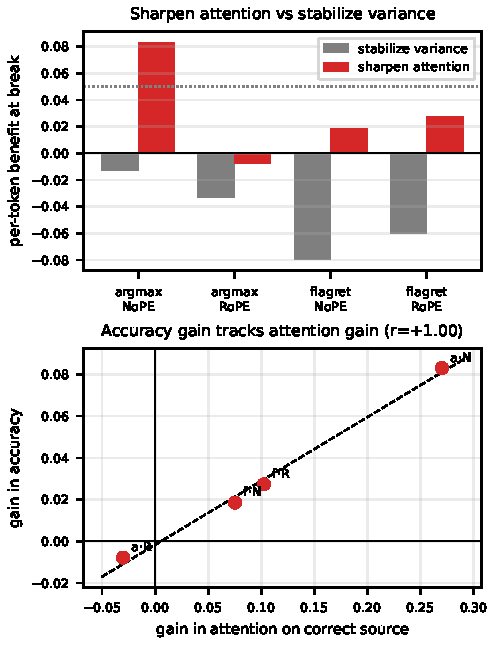
\includegraphics[width=0.82\textwidth]{figures/fig_intervention.pdf}
\caption{The intervention test.
Top: per-token benefit at the break point for stabilizing variance (gray) and sharpening attention (red),
by cell, with the dotted line at the pre-registered threshold of $0.05$.
Bottom: across the four cells the accuracy gain from sharpening tracks the gain in attention on the correct
source, with correlation $+1.0$.
Raising the operative variable raises accuracy, and the variance-stabilizing intervention raises neither.}
\label{fig:intervention}
\end{figure*}

We report the strength of the effect plainly.
The single log-length lever is a partial rescue.
Its per-token gain at the break point clears our pre-registered threshold of $0.05$ on argmax under NoPE,
where it reaches $+0.083$ across four seeds, and it is smaller on the other cells.
A full recovery of short-length accuracy would need more than one inference-time knob \citep{sparselong}.
The interventional result confirms the direction of the account, that attention selection is the operative
lever, and it leaves the size of the achievable rescue to stronger concentration methods.

\subsection{Fixed-spectrum assignment}
\label{sec:permutation}

Sharpening changes the attention spectrum and the assignment together.
To isolate assignment, we permute each selected attention row at the answer query while leaving its multiset
of weights fixed.
The source-max condition swaps the source weight with the row maximum, the source-min condition swaps it
with the row minimum, and the distractor control swaps the largest and smallest non-source weights.
All conditions preserve entropy, every attention norm, the maximum weight, participation ratio, and the
complete sorted distribution exactly.

We select one retrieval layer and rank its heads using only training-length examples, then freeze that
choice for evaluation at lengths $100$ and $250$.
Across the sixteen task, positional-encoding, and seed cells, patching all eight heads with source-max raises
per-token accuracy by $0.153$ (95\% bootstrap interval $[0.086,0.222]$).
Source-min lowers it by $0.043$ ($[-0.058,-0.030]$), while the distractor control changes it by $0.011$
($[0.004,0.018]$).
Source-max exceeds the distractor control in all $32$ model--length comparisons, with a paired difference of
$0.142$ ($[0.081,0.205]$), and source-min is negative in all $32$.

The effect also has the head-dose structure predicted by Theorem~\ref{thm:nonlinear-margin}.
The mean source-max gain rises from $0.007$ with one patched head to $0.013$, $0.056$, and $0.153$ with two,
four, and eight heads, monotone in $31$ of the $32$ model--length comparisons.
The sorted-spectrum error is numerically zero and every derived invariant error is below $10^{-6}$.
These interventions instantiate the fixed-spectrum routing range: the concentration capacity is unchanged,
and accuracy follows which token receives it.

The fixed-spectrum intervention establishes that assignment matters at one natural spectrum; a full test of
the decomposition must vary capacity and assignment independently.
We therefore apply temperatures $\beta\in\{1,2,4\}$ to each natural row and, at every resulting spectrum,
compare the identity assignment, source-max, source-min, and the distractor-only control.
Across all sixteen trained models, sharpening raises the mean maximum weight from $0.362$ to $0.655$.
The source-max minus source-min accuracy contrast grows from $0.196$ at $\beta=1$ to $0.346$ at $\beta=4$,
an interaction of $+0.151$ (95\% bootstrap interval $[0.094,0.210]$), positive in $15$ of $16$ models.
By contrast, sharpening the identity assignment changes accuracy by only $+0.007$ at $\beta=2$ and
$+0.009$ at $\beta=4$.
Capacity and assignment are therefore not rival descriptions: greater selective capacity increases the
behavioral leverage of where the spectrum is assigned, but capacity alone does not select the source.

We next test the value-utility condition in Theorem~\ref{thm:nonlinear-margin}, rather than inferring it from
accuracy.
For every example and head, we continuously interpolate the source-max swap from its natural row and
differentiate the target-versus-strongest-competitor margin at the natural endpoint.
The resulting first-order term is exactly the transferred source mass times the local source-versus-
distractor utility gap.
Across $1{,}024$ examples from the same sixteen models, that term predicts the exact finite source-max
margin change with pooled Pearson correlation $0.917$, Spearman correlation $0.989$, and $99.5\%$ sign
agreement (Figure~\ref{fig:capacity-assignment}, right).
The correlation between cell-mean predicted and actual changes is $0.978$.
Active source utility gaps are positive in $89.2\%$ of head-example pairs; the remaining cases and a mean
absolute nonlinear residual of $1.19$ mark the theorem's intended boundary rather than being hidden by an
average effect.
Source-max raises answer accuracy from $0.239$ to $0.533$ in this audit.

\begin{figure*}[t]
\centering

\includegraphics[width=0.96\textwidth]{figures/fig_capacity_assignment.pdf}
\caption{Independent tests of the capacity--assignment decomposition.
Left: sharpening increases the maximum available attention weight, and the source-max versus source-min
accuracy contrast grows with it; sharpening without reassignment remains near zero.
Right: at the cell level, the theorem's first-order routing term predicts the exact source-max change in the
target-versus-competitor output margin across tasks and positional encodings.
Error bars are 95\% bootstrap intervals over models.}
\label{fig:capacity-assignment}
\end{figure*}

\subsection{Routing a two-token evidence set}
\label{sec:multi-evidence}

The preceding interventions use tasks whose answer is available at one source position.
We test Corollary~\ref{cor:multi-evidence} on a task that requires two values.
Each sequence contains decimal digits, two independently marked positions, and an answer query whose target
is the sum of the marked digits modulo ten.
Copying either marked digit is insufficient.
We train two-layer, width-$128$, four-head models at lengths up to five with NoPE or RoPE and four seeds per
encoding.
All eight models reach perfect train-length exact match, satisfying the competence gate before intervention.

At one head selected using train-length evidence mass, evidence-max assigns the two largest weights to the
two marked positions with the minimum number of swaps.
Evidence-min analogously assigns the two smallest weights.
The distractor control swaps non-evidence weights while preserving both the complete attention spectrum and
the total evidence mass.
The interventions reuse $256$ paired examples per model and length.

\begin{table}[H]
\centering
\small
\resizebox{\columnwidth}{!}{%
\begin{tabular}{lrrrrr}
\toprule
Length & Natural & Evid.-max & Evid.-min & Control & Max--ctrl. \\
\midrule
$2\times$ & $0.952$ & $0.971$ & $0.393$ & $0.964$ & $+0.007$ \\
$5\times$ & $0.484$ & $0.550$ & $0.194$ & $0.507$ & $+0.043$ \\
\bottomrule
\end{tabular}
}
\caption{Exact match on two-evidence modular sum, averaged over eight competent models.
At $5\times$ length, evidence-max minus control has a 95\% paired bootstrap interval of
$[0.017,0.072]$; evidence-max minus evidence-min is $+0.356$ ($[0.257,0.450]$).}
\label{tab:multi-evidence}
\end{table}

At $5\times$ length, evidence-max raises exact match over the natural model by $0.066$
($[0.043,0.091]$), evidence-min lowers it by $0.291$ ($[-0.395,-0.186]$), and the control changes it by
$0.023$ ($[0.006,0.042]$).
Evidence-max exceeds the evidence-mass-preserving control by $0.043$ ($[0.017,0.072]$) and evidence-min by
$0.356$ ($[0.257,0.450]$).
The max--min contrast is positive in every model, and max--control is positive in seven of eight.
Every selected-head condition preserves the sorted spectrum exactly; the largest derived-invariant error is
$4.77\times10^{-7}$.
The result extends the assignment law from a single copied source to a learned two-input computation while
leaving the boundary in Section~\ref{sec:limitations} explicit.

\subsection{A forced-mass dose response}
\label{sec:patch}

The sharpening intervention changes the attention logits, so it is an indirect test.
We also manipulate the operative variable directly.
At the answer-query position we overwrite the attention distribution to place a chosen mass on the correct
source, holding the trained weights fixed, and read the accuracy.
The construction and the pre-registration are released with the paper.

Forcing attention onto the correct source restores accuracy (Figure~\ref{fig:patch}, top).
At $50\times$ the training length, where the baseline sits at $0.59$ per token, patching the attention to
attend fully to the source raises accuracy to $0.99$, and the effect is monotone in the forced attention.
Fifteen of the sixteen cells reach near $1.0$, and the one exception is argmax under RoPE, the cell that
also resisted sharpening.
Accuracy rises with the forced attention on the source across the sweep at a held attention norm, with
correlation $0.89$ (Figure~\ref{fig:patch}, bottom).

\begin{figure*}[t]
\centering

\includegraphics[width=0.82\textwidth]{figures/fig_patch.pdf}
\caption{Direct manipulation of the operative variable, pooled over the sixteen models at $50\times$.
Top: patching the answer-query attention to place mass on the correct source restores accuracy from the
baseline (dotted) to near $1.0$, monotone in the forced attention.
Bottom: with the attention norm held by construction, accuracy rises with attention on the correct source
(correlation $0.89$).}
\label{fig:patch}
\end{figure*}

We state the limits of this manipulation.
It shows that attention on the correct source is sufficient to drive the readout, since forcing it restores
accuracy and starving it returns accuracy to chance.
It does not hold the attention-output variance exactly constant, because the source value vector is not
exchangeable with the others, so the measured variance still drifts as the attention concentrates.
The manipulation therefore demonstrates the sufficiency of selection, and we do not read it as a proof that
the variance is causally inert.

\section{Generalization across pretrained model families}
\label{sec:realmodel}

The results so far are on small transformers trained from scratch.
We ask whether source-labeled routing remains informative in pretrained models with different architectures
and training histories.
We probe Pythia-1.4B, Qwen2.5-1.5B, and Gemma-2-2B on in-context key-value recall: the prompt lists pairs in
the form
\texttt{key: value}, a query repeats one key, and the model should produce the paired value.
The value's position is known, so we read attention on the correct source, and we vary the number of pairs
as the context length.
A pretrained model routes retrieval through specific heads, so we select the $K$ heads with the highest
source attention at the shortest length and freeze that set across the sweep.
We use $K=8$ for the cross-model comparison and vary $K$ for Qwen as a robustness check.

Table~\ref{tab:realmodel-family} and Figure~\ref{fig:realmodel} show two regimes.
Pythia and Qwen cross into failure as context grows: accuracy drops by $0.493$ and $0.760$, while selected-
head source attention drops by $0.259$ and $0.356$.
Gemma is the informative boundary case.
Its mean source attention still drops by $0.250$, but accuracy remains approximately flat
($0.507$ to $0.513$), so mean source-attention decline is not itself sufficient for failure.
Within each fixed length, however, Gemma examples with more source attention are more often correct: the
mean point-biserial correlation is $0.346$, above participation ratio at $0.268$ and negative entropy at
$0.238$, and source attention wins at all six lengths.
The corresponding source-attention correlations are $0.194$ for Pythia and $0.268$ for Qwen with eight
heads; varying Qwen from four to sixteen heads preserves the result, with source attention the strongest
candidate at eight and sixteen heads and narrowly behind negative entropy at four.
Thus source-labeled routing is the strongest within-length candidate in four of five probes, while whether
its lengthwise decline becomes an aggregate accuracy failure depends on the model's available margin and
downstream readout.

\begin{table*}[t]
\centering
\small
\begin{tabular}{lrrrrrrl}
\toprule
Model & $K$ & $\Delta$Acc. & $\Delta$Src. attn. & $r_{\mathrm{src}}$ & $r_{\lVert a\rVert_2^2}$ & $r_{-H}$ & Winner \\
\midrule
Pythia-1.4B & 8  & $-0.493$ & $-0.259$ & $0.194$ & $0.122$ & $0.100$ & source \\
Qwen2.5-1.5B & 4  & $-0.760$ & $-0.370$ & $0.219$ & $0.214$ & $0.231$ & $-H$ \\
Qwen2.5-1.5B & 8  & $-0.760$ & $-0.356$ & $0.268$ & $0.223$ & $0.248$ & source \\
Qwen2.5-1.5B & 16 & $-0.760$ & $-0.295$ & $0.317$ & $0.176$ & $0.246$ & source \\
Gemma-2-2B & 8 & $+0.007$ & $-0.250$ & $0.346$ & $0.268$ & $0.238$ & source \\
\bottomrule
\end{tabular}
\caption{Pretrained-model family probe from five to $160$ key--value pairs.
Changes are last minus first length; correlations are means of within-length point-biserial correlations
with answer correctness, avoiding length as a common cause.
Source attention wins four of five head-set probes, while Gemma shows that a declining mean need not cross
the model's failure threshold.}
\label{tab:realmodel-family}
\end{table*}

\begin{figure*}[t]
\centering

\includegraphics[width=0.96\textwidth]{figures/fig_realmodel_family.pdf}
\caption{In-context key--value recall across pretrained model families.
Left: Pythia and Qwen cross into failure as context grows, while Gemma accuracy remains approximately flat.
Right: selected-head attention on the correct source declines in all three models.
Gemma separates a routing-pressure diagnostic from a universal failure law: lower mean source attention
need not impair accuracy until the downstream margin is exhausted.}
\label{fig:realmodel}
\end{figure*}

\subsection{Fixed-spectrum causality in a pretrained model}
\label{sec:pretrained-causal}

The observational comparison does not isolate assignment from correlated properties of a natural
attention row. We therefore apply the same fixed-spectrum test inside Qwen2.5-1.5B. On 64 calibration
examples at five pairs, we select the layer and four heads with the highest source mass, then freeze that
choice across lengths. For each of 128 paired examples per length, source-max swaps the source weight with
the row maximum, source-min swaps it with the row minimum, and the control swaps the largest and smallest
distractor weights without changing the source. All conditions use the same prompts and model weights.

Table~\ref{tab:pretrained-causal} shows the result. Source-max raises accuracy at every length, with paired
$95\%$ bootstrap intervals excluding zero, and raises the correct-answer margin by $1.177$--$2.527$ logits.
Against the matched distractor-only permutation, source-max raises accuracy by $0.117$, $0.164$, $0.109$,
and $0.062$; the four paired intervals exclude zero.
Source-min lowers the margin at every length and lowers accuracy whenever the baseline is above its floor.
At 80 and 160 pairs the distractor-only control changes accuracy by exactly zero, while source-max still
raises it by $0.109$ and $0.062$. The maximum discrepancy in any permutation-invariant diagnostic is
$4.77\times10^{-7}$. Thus, in a pretrained model with nontrivial short- and intermediate-length competence,
the location of a fixed set of attention weights causally changes the output; concentration alone cannot
identify that location. This is one model-family causal replication, not evidence that the effect size is
universal across architectures.

We repeat the intervention in Qwen2.5-7B using NF4 weights with bfloat16 computation and 96 paired examples
per length. Source-max minus control raises the output margin by $0.185$, $0.747$, and $0.773$ at five, 20,
and 80 pairs, with intervals $[0.040,0.363]$, $[0.476,1.048]$, and $[0.549,1.047]$. At 20 pairs it also
raises accuracy over control by $0.125$ ($[0.062,0.198]$). The five-pair accuracy interval crosses zero,
and the 80-pair baseline is $0.010$, leaving accuracy floor-limited even though the margin moves. The margin
result therefore replicates across scale within Qwen; we next test whether it crosses architecture families.

We then repeat the same test in Pythia-1.4B with 128 paired examples per length. At five pairs, where
baseline accuracy is $0.359$, source-max exceeds the distractor control by $0.070$ accuracy
($[0.016,0.133]$) and $0.639$ margin ($[0.400,0.887]$); source-min lowers baseline accuracy by $0.250$ and
margin by $2.480$. At 20 pairs, source-max still exceeds control by $0.055$ accuracy
($[0.016,0.102]$) and $1.097$ margin ($[0.905,1.309]$), although baseline accuracy has fallen to $0.039$.
At 80 pairs baseline accuracy is exactly zero, so accuracy cannot identify an effect, but source-max still
exceeds control by $0.306$ margin ($[0.185,0.424]$). Source-min no longer has a negative margin effect in
that floor-saturated cell. The source-max assignment-margin prediction therefore replicates across Qwen2
and GPT-NeoX architectures; the full bidirectional accuracy asymmetry is supported where the natural model
retains enough competence to cross the decision boundary.

Gemma-2-2B supplies a third-architecture boundary with 128 paired examples per length. Its baseline accuracy
remains between $0.711$ and $0.758$ from five to 80 pairs, and its natural selected-head source mass remains
high, declining from $0.670$ to $0.440$. Source-max adds another $0.059$--$0.129$ source mass but is neutral
against the distractor control: all three accuracy and margin intervals include zero. Source-min removes
almost all source mass and lowers accuracy by $0.094$, $0.133$, and $0.117$, with intervals
$[-0.164,-0.023]$, $[-0.203,-0.062]$, and $[-0.180,-0.062]$. It lowers the output margin by $1.680$,
$1.341$, and $1.096$, again with all intervals excluding zero. Gemma therefore rejects a universal
monotone claim that more source mass must improve behavior. It supports the conditional theorem: assignment
is causal when it removes useful routed evidence, while additional routing can be redundant once the model's
available output margin is already sufficient.

We directly audit the theorem's utility condition inside all three pretrained architectures.
On 64 independently evaluated examples at each of five and 20 pairs, we interpolate continuously from the
natural attention row to each fixed-spectrum swap and differentiate the target-versus-fixed-competitor
margin at the natural endpoint.
For source-max, the first-order term predicts the exact finite effect with Spearman correlations
$0.798$ and $0.866$ in Qwen, $0.647$ and $0.448$ in Pythia, and $0.496$ and $0.572$ in Gemma.
The corresponding sign-agreement rates range from $0.703$ to $0.812$.
The same audit predicts the negative mean source-min effect in every model--length cell.
Gemma's source-max effect is small in both the local and exact calculations, while its source-min effect is
large, so its asymmetric boundary is explained by downstream utility and saturation, and the assignment
intervention retains the predicted direction.

We repeat the complete utility audit with seeds 1 and 2 for all three models. Across seeds $0,1,2$, the
source-max first-order/exact association is positive in all six model--length cells for each model. The mean
seed-level Spearman correlation is $0.866$ for Qwen ($95\%$ interval $[0.832,0.898]$), $0.544$ for Pythia
($[0.500,0.586]$), and $0.554$ for Gemma ($[0.534,0.582]$), with mean sign agreement $0.805$, $0.807$, and
$0.714$. Gemma's mean exact source-max effect remains only $+0.050$, preserving its saturation boundary even
though the local association replicates.

We also repeat circuit selection on an independent calibration split for three seeds and
$K\in\{2,4,8\}$ in Qwen at 20 pairs.
All nine selected seed-by-$K$ cells have a positive source-max versus distractor-control margin, and every
paired $95\%$ interval excludes zero.
Their mean margin effect is $+0.874$, compared with $-0.059$ for one deterministic random-layer control per
seed and $+0.008$ across the adjacent-layer controls.
The selected layer is 14 in every calibration, while the random layers vary from 7 to 21.
The result therefore survives independent calibration and evaluation examples, head count, and seed, and
it localizes the effect more sharply than selecting an arbitrary layer.

We then run two preregistered external-validity checks. A blinded baseline-only pilot selects the
\texttt{arrow\_newline} format, but its seed-zero full run falls to $0.156$, $0.117$, and $0.008$ accuracy at
five, 20, and 80 pairs, so it fails the locked competence gate. The causal signs nevertheless remain
directional: source-max minus control raises margin by $4.633$, $3.558$, and $0.674$, while source-min lowers
it by $1.086$, $0.893$, and $0.240$. We therefore do not claim a competent second-format replication.

For the Llama-family check, SmolLM2-1.7B passes the locked pilot and intervention backend, then reaches
$0.945$, $0.516$, and $0.023$ baseline accuracy in the 128-example full run. Source-min lowers margin in the
two competent cells, by $0.133$ and $0.190$, but source-max minus the matched distractor control changes
margin by $-0.018$, $-0.199$, and $-0.056$ from shortest to longest. The preregistered source-max gate thus
fails. This does not contradict Theorem~\ref{thm:nonlinear-margin}: the guarantee requires positive
source-versus-donor downstream utility, whereas these heads were selected only by natural source mass. It
does rule out treating high source mass as an architecture-independent intervention-selection criterion.

\paragraph{Utility-conditioned rescue.}
We lock a follow-up before observing its outcomes: on an independent 64-example calibration split, score
every head by the theorem's first-order source-max term---available transferred mass times the local
source-versus-donor margin-utility gap---then choose the layer with the largest top-four score sum. We
compare this rule with the original source-mass selector on the same 128 evaluation examples for each of
three seeds. At five pairs, pooled untouched accuracy is $0.956$. Utility-selected source-max exceeds the
spectrum-matched control by $0.702$ margin ($95\%$ CI $[0.529,0.858]$) and $0.052$ accuracy;
source-mass selection changes margin by $-0.021$ ($[-0.057,0.014]$). The paired
utility-minus-mass effect is $+0.723$ ($[0.544,0.882]$). These intervals resample calibration seeds and
paired examples within each sampled seed. The utility rule selects layer 8 in seed zero and
layer 15 in seeds one and two, so the replication tests a selection rule rather than one fixed circuit.
At 20 pairs the utility margin effect remains positive in every seed and pools to $+2.200$
($[1.920,2.493]$), but pooled baseline accuracy is $0.432$, below the locked $0.50$ competence gate; we
treat it as margin-only evidence. Seed zero supplies the optional 80-pair diagnostic, where baseline
accuracy is $0.023$ and the margin effect is $+0.163$ ($[0.059,0.291]$). Thus the competent primary test
passes without converting low-competence tails into behavioral evidence.

We next test selector specificity with the same calibration and evaluation budgets over ten seeds.
The comparison includes source mass, available transfer mass, utility gap, predicted utility gain,
source gradient, gradient magnitude, and a deterministic random circuit.
Source-gradient selection ranks first with a mean source-max-minus-control margin of $+0.750$
(calibration-seed bootstrap interval $[0.682,0.819]$), followed by utility gain at $+0.600$
($[0.482,0.712]$) and utility gap at $+0.296$ ($[0.232,0.354]$).
Source mass is $-0.040$ and random selection is $-0.019$.
Utility gain trails source gradient by $0.150$ ($[-0.274,-0.026]$ for utility minus source gradient), so
the preregistered utility-specificity rule fails.
The broader result is that task-conditioned output sensitivity identifies useful circuits more reliably
than task-agnostic attention mass in this model and task.

We also interpolate continuously from each natural attention row to the complete utility-selected swap,
with a displacement-matched distractor interpolation as control.
Across five independent calibration seeds, the mean source-minus-control margin is $0.000$, $0.446$,
$0.817$, $1.128$, and $1.417$ at interpolation strengths $0$, $0.25$, $0.5$, $0.75$, and $1$.
Every seedwise path is nondecreasing, and the hierarchical endpoint interval is $[1.332,1.514]$.
The effect therefore develops smoothly along the intervention path and is not confined to the maximal swap.

We then amend the failed open-answer SQuAD protocol before observing follow-up intervention outcomes.
The amended test uses four-choice natural questions, retains only examples answered correctly with the
passage and gold passage alone but incorrectly without context, and freezes disjoint calibration and
evaluation sets before intervention. In the locked 64-calibration/128-evaluation design, full-context
rescue on no-context failures is $0.981$, $0.966$, and $0.951$ across three seeds.
Utility-selected source-max exceeds the spectrum-matched control by $+0.336$ margin with a hierarchical
$95\%$ interval $[0.176,0.512]$ and raises unconstrained next-token accuracy by $+0.008$
($[0.000,0.021]$). Source-mass selection is harmful at $-0.112$ ($[-0.188,-0.043]$).
An eight-token greedy-decoding audit changes neither first-answer accuracy nor repetition relative to control.

We next freeze the utility-selected circuit at four passages and append unrelated natural passages without
changing the gold passage, answer options, or existing distractors. Two full Qwen seeds show a 4-to-32
passage margin change of $-1.036$ ($[-1.397,-0.698]$) and accuracy change of $-0.047$
($[-0.074,-0.023]$). However, source mass increases by $0.00095$ and the source-max-minus-control effect
weakens by $-0.179$ ($[-0.352,-0.005]$), opposite to the proposed rescue-amplification mechanism.
A frozen SmolLM2 replication also loses margin ($-0.193$) and accuracy ($-0.102$); its source mass declines,
but rescue amplification is null at $+0.018$ ($[-0.027,0.066]$). Thus natural context length reliably hurts
performance here, while source-mass loss is neither necessary nor sufficient to explain that effect.

Finally, an equal-budget selector-family test uses 64 calibration and 128 evaluation examples over three
seeds each. Utility gain ranks first on Pythia-1.4B ($+0.519$) and SmolLM2-1.7B ($+1.253$), but ranks
second on Qwen2.5-1.5B, where utility gap, utility gain, and source gradient select the same effective
circuit and tie near $+1.49$. The strict universal-selector criterion therefore fails, while the broader
output-conditioned-selection result replicates across all three families.

\begin{table*}[t]
\centering
\small
\begin{tabular}{lrrrrrrr}
\toprule
Model & $N$ & Base & \multicolumn{3}{c}{$\Delta$ accuracy} & \multicolumn{2}{c}{$\Delta$ margin} \\
\cmidrule(lr){4-6}\cmidrule(lr){7-8}
& & Acc. & Src.-max & Src.-min & Control & Src.-max & Src.-min \\
\midrule
Qwen-1.5B & 5   & .539 & $+.102$ & $-.258$ & $-.016$ & $+1.177$ & $-1.406$ \\
& 20  & .398 & $+.188$ & $-.117$ & $+.023$ & $+2.268$ & $-1.191$ \\
& 80  & .070 & $+.109$ & $-.023$ & $+.000$ & $+2.527$ & $-.285$ \\
& 160 & .008 & $+.062$ & $+.000$ & $+.000$ & $+2.204$ & $-.148$ \\
\midrule
Qwen-7B NF4 & 5  & .448 & $+.021$ & $-.135$ & $+.010$ & $+.325$ & $-.988$ \\
& 20 & .271 & $+.135$ & $-.104$ & $+.010$ & $+.891$ & $-1.185$ \\
& 80 & .010 & $+.010$ & $-.010$ & $+.000$ & $+.654$ & $-.546$ \\
\midrule
Pythia-1.4B & 5  & .359 & $+.109$ & $-.250$ & $+.039$ & $+.878$ & $-2.480$ \\
& 20 & .039 & $+.039$ & $-.039$ & $-.016$ & $+1.195$ & $-.622$ \\
& 80 & .000 & $+.000$ & $+.000$ & $+.000$ & $+.405$ & $+.034$ \\
\midrule
Gemma-2-2B & 5  & .758 & $+.008$ & $-.094$ & $+.016$ & $+.041$ & $-1.680$ \\
& 20 & .711 & $+.016$ & $-.133$ & $-.008$ & $+.020$ & $-1.341$ \\
& 80 & .742 & $+.000$ & $-.117$ & $+.000$ & $+.058$ & $-1.096$ \\
\midrule
SmolLM2-1.7B & 5  & .945 & $+.008$ & $-.008$ & $-.008$ & $-.013$ & $-.133$ \\
& 20 & .516 & $-.016$ & $+.000$ & $+.008$ & $-.410$ & $-.190$ \\
& 80 & .023 & $+.000$ & $+.000$ & $+.000$ & $-.083$ & $-.012$ \\
\bottomrule
\end{tabular}
\caption{Paired fixed-spectrum interventions in Qwen2.5 at two scales, Pythia-1.4B, Gemma-2-2B, and
SmolLM2-1.7B, with
128 examples per length except 96 for Qwen-7B.
Source-max accuracy-gain intervals are $[.055,.156]$, $[.125,.258]$, $[.055,.164]$, and $[.023,.109]$
from shortest to longest. Source-max minus control intervals are $[.055,.188]$, $[.102,.234]$,
$[.055,.164]$, and $[.023,.109]$. The control preserves source assignment as well as the spectrum.
SmolLM2 is the preregistered negative replication: source-max does not beat its matched control.}
\label{tab:pretrained-causal}
\end{table*}

\subsection{Decomposing the failure: attention and readout}
\label{sec:decouple}

We perform this additional decomposition on Pythia, where the required intermediate logit-lens artifacts
were recorded.
Its co-decline localizes part of the failure to attention, and attention on the source is still non-trivial
where accuracy is low, so we ask whether attention is the whole story.
At the query token we read three things: whether attention reached the source (retrieval-head attention on the
correct source), whether the value was retrieved into the residual stream (the correct value appears in the
top ten of a logit lens at some layer, using the model's own final norm and unembedding), and whether the
value was output (the answer is correct).
Among the failures at each length we separate two loci.
A failure is attention-limited when the value is absent from the residual and attention on the source is low.
A failure is readout-limited when the value is present in the residual yet the model does not output it, so a
competing token wins after a successful retrieval.

The failure is not attention alone (Figure~\ref{fig:decouple}).
At moderate length the failures are predominantly readout-limited, from $0.95$ of failures at ten pairs to
$0.58$ at eighty, where the model retrieves the value and then loses it to a distractor.
Attention-limited failures grow with length, from $0.05$ to $0.60$ over the same range, and become the
majority only at the longest context.
The two loci cross near the longest length we test.
Attention on the correct source is therefore the dominant failure at the largest contexts, in agreement with
the operative-variable account at the tail, while a downstream readout locus carries most of the failure at
moderate length.
The split is robust to the thresholds, with the readout share at the longest length between $0.34$ and $0.50$
across the ranges we tried, and the logit lens counts a value as present leniently, so the readout share is a
lower bound.

\begin{figure*}[t]
\centering
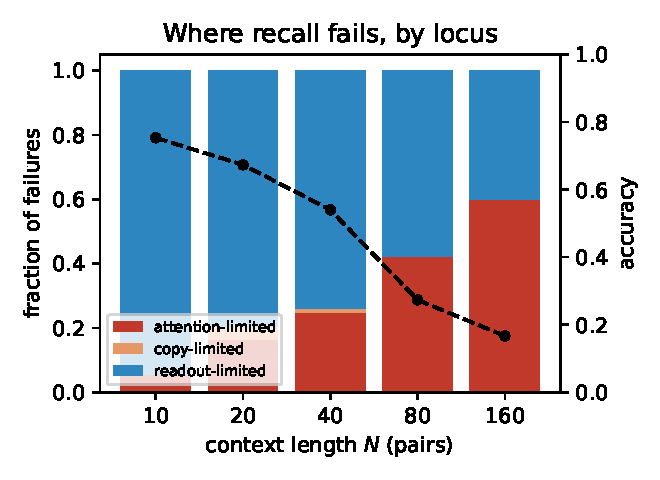
\includegraphics[width=0.82\textwidth]{figures/fig_decouple.pdf}
\caption{Where in-context recall fails in Pythia-1.4B, by locus, among the failures at each length.
Readout-limited failures, where the correct value is in the residual yet not output, dominate at moderate
length; attention-limited failures, where attention never reaches the source, grow with length and become the
majority at the longest context. Dashed line: accuracy.}
\label{fig:decouple}
\end{figure*}

\section{Limitations}
\label{sec:limitations}

The models are small.
We report at four layers and width $256$, and we replicate the full result at eight layers and width $512$
(Section~\ref{sec:res-scale}), which is roughly eight times the parameters, and we do not reach frontier
scale.
We do not observe a length-generalization improvement from holding the variance constant at either size,
and we cannot exclude that a much larger model or a different task construction behaves differently.

Our identification of task-correct assignment rests on direct measurement and matched interventions.
The spectrum-preserving test isolates assignment in the controlled models, while the sharpening correlation
is measured over four cells and remains suggestive at the population level.
The affine routing theorem assumes a linear downstream margin, and the nonlinear guarantee requires a
positive source-value utility gap and bounded downstream curvature along the intervention path.
Our gradient audit measures the local utility term and its finite-intervention residual, but it does not
estimate a Lipschitz constant or provide a per-example curvature certificate.
Positive utility holds in $89.2\%$, not all, active head-example pairs, and the nonzero residual means the
first-order prediction is not a globally linear model of the intervention.
The account is stated for events with identifiable evidence positions.
The two-evidence modular-sum experiment shows that the set-valued law can govern a learned computation, but
evidence availability remains only a necessary condition for unrestricted computation. A registered
two-/three-/four-evidence stage finds perfect train competence at $r=2,3$, but no positive max--control
interval at $r=3$; at $r=4$, minimum train exact match falls to $0.090$. Thus the present causal
generalization stops at $r=2$ and does not cover arbitrary evidence arity or long intermediate computations.
The order-dependent contrast further shows that the same treatment does not automatically cover tasks
whose routing requirements change across output positions.
The tasks are synthetic and chosen for control, so they isolate the mechanism and are not a measure of
end-task benchmark performance.
The pretrained observational probe covers three open-weight model families but only one synthetic in-context
retrieval task. The pretrained causal result covers Qwen2.5 at two scales, Pythia-1.4B, Gemma-2-2B, and
SmolLM2-1.7B, spanning Qwen2, GPT-NeoX, Gemma2, and Llama architectures.
A preregistered equals-sign prompt variant retains the predicted intervention directions at five and 20
pairs, but Qwen baseline accuracy is only $0.164$ and $0.203$, so it fails the competence gate and cannot
support a second-format causal replication.
Its 80-pair cell is also below competence. A blinded pilot selected an arrow-delimited variant, and its
source-max and source-min margin signs replicate at all three lengths, but the seed-zero full run again
fails competence. The second-format claim therefore remains open.
The 7B run is quantized, and
accuracy is floor-limited at the longest context. Pythia-1.4B also reaches the accuracy floor by the longest
context, so its tail supports the margin prediction without testing accuracy rescue. Gemma provides a
high-competence boundary where source-min is causal but source-max is redundant. The Pythia-70M run validates
the backend but lacks sufficient baseline competence and is not treated as substantive evidence. SmolLM2
passes the Llama-family competence and backend gates, but fails the source-max gate under natural-source-mass
head selection. A separately preregistered utility-gain selector rescues the competent five-pair condition
across three seeds, while its 20-pair replication is margin-only because pooled baseline accuracy misses the
competence gate and its 80-pair diagnostic is available only for seed zero. A ten-seed selector ablation
places source gradient above utility gain. The three-family follow-up likewise finds utility gain first on
Pythia and SmolLM but tied behind utility gap under Qwen's frozen ordering. Thus the result supports
output-conditioned circuit selection without establishing one universal formula.
The amended natural multiple-choice QA protocol passes its locked 64/128 fixed-context design over all three
seeds, but its positive intervention result does not extend to the nested length ladder: Qwen and SmolLM2
both degrade with length without a shared source-mass-loss or increasing-rescue mechanism. The
variable-evidence stage does not extend the positive causal result beyond two sources: the three-source
interval includes zero, and all preregistered four-source capacity candidates fail competence. The largest
candidate reaches $0.748$ exact match against the frozen $0.8$ gate, so no four-source causal contrast is
interpreted.
Pythia and Qwen show a co-decline, whereas Gemma retains accuracy despite lower mean source attention; this
rules out a model-independent mean-attention threshold and supports only the within-length routing claim.
The Pythia-only failure decomposition uses a logit lens, which reads intermediate residuals imperfectly and
counts a value as present leniently, so the readout locus is a lower bound and the split is a characterization
of this model and task.
Most synthetic-task accuracy is measured with teacher forcing per token, an upper bound on free generation;
the full-size natural-QA audit additionally performs unconstrained eight-token greedy decoding.
Dictionary lookup did not reach our competence gate at this scale and is reported as untrained.

\section{Conclusion}
\label{sec:conclusion}

We asked which internal property supports transformer length generalization on retrieval, and we answered
by direct measurement.
Attention on the correct source token predicts accuracy with correlation $0.97$, across tasks and
positional encodings, and generalization holds while that attention stays concentrated and fails as it
disperses.
A natural alternative, the scale of the attention output, collapses with length as well, predicts accuracy
less well, and does not transfer to the behavior when an intervention holds it constant, with a cost under
rotary position embeddings.
Raising attention on the correct source by inference-time sharpening raises accuracy in proportion, while
stabilizing the scale raises neither.
At a fixed attention spectrum, assigning the maximum weight to the source raises accuracy by $0.153$,
assigning the minimum lowers it by $0.043$, and permuting distractors alone changes it by $0.011$.
A capacity-by-assignment factorial strengthens the causal result: the correct-versus-wrong assignment
contrast grows by $0.151$ as the spectrum sharpens, while sharpening without reassignment changes accuracy
by at most $0.009$.
The theorem's first-order utility-gap term predicts the exact finite output-margin change over $1{,}024$
examples with correlation $0.92$ and $99.5\%$ sign agreement, while its failures and nonlinear residual
make the value/readout boundary explicit.
The same local term predicts exact source-max swap effects inside Qwen, Pythia, and Gemma, with positive
Spearman association in all six model--length cells.
Across Qwen, Pythia, and Gemma, the association remains positive in all eighteen source-max
model--length--seed cells across three seeds, while the preregistered SmolLM2 source-max replication fails,
preserving the theorem's conditional form and rejecting a universal source-mass head-selection rule.
Replacing that selector with independently calibrated first-order utility gain rescues SmolLM2 at the
competent five-pair condition across three seeds: the pooled source-max-minus-control margin is $+0.702$
and the paired advantage over source-mass selection is $+0.723$, with both intervals excluding zero.
A ten-seed equal-budget ablation sharpens the scope: source gradient ranks first at $+0.750$, utility gain
second at $+0.600$, and source mass remains negative at $-0.040$.
The restored five-seed interpolation path rises monotonically in every seed from zero contrast to $+1.417$, which
supports a graded routing effect instead of a maximal-swap artifact.
The same fixed-spectrum prediction survives a two-evidence computation: at $5\times$ length, assigning the
top-two weights to the marked evidence raises exact match by $0.066$, assigning the bottom two lowers it by
$0.291$, and evidence-max exceeds an evidence-mass-preserving distractor control by $0.043$.
Patching the attention directly onto the correct source restores accuracy from $0.59$ to near $1.0$ in these
models and tasks.
Across three pretrained model families, source-labeled attention is the strongest within-length predictor
in four of five probes.
Pythia and Qwen cross into failure as source attention declines; Gemma does not, showing that routing
pressure becomes failure only when it exhausts a model- and task-dependent output margin.
In Qwen2.5-1.5B, a paired fixed-spectrum intervention then assigns the model's existing maximum attention
weight to the source and raises accuracy at every tested length, while source-min moves the output margin in
the opposite direction. Qwen2.5-7B replicates the source-max versus control margin effect at every tested
length, including where raw accuracy reaches its floor. Pythia-1.4B replicates the assignment-margin effect
across architecture families and the accuracy asymmetry where it remains competent. Gemma-2-2B then supplies
the necessary boundary: removing source mass harms behavior, while adding more is redundant in a model that
remains competent. Independent Qwen calibrations preserve the source-max versus control margin effect for
all three seeds and all three tested head counts. Together these results support a conditional routing law
without mistaking it for universal monotonicity.
An amended context-dependent SQuAD multiple-choice test passes its locked 64/128 design over three seeds:
utility-selected source-max exceeds matched control by $+0.336$ margin ($[0.176,0.512]$), while source-mass
selection is significantly negative. The greedy-decoding audit shows no repetition or first-answer cost.
A nested 4--32-passage follow-up establishes natural-QA length degradation in Qwen and SmolLM2, but its
stronger mechanistic prediction fails: Qwen source mass rises and rescue weakens, whereas SmolLM2 source mass
falls without increasing rescue. The result therefore broadens the behavioral length effect while narrowing
the causal claim back to the tested fixed-context and synthetic settings.
A three-family selector comparison rejects a unique universal selector while retaining the broader
output-conditioned-circuit claim. A registered arity extension supplies a boundary rather than a positive
generalization: three-source max--control includes zero, and the largest four-source capacity candidate
reaches only $0.748$ exact match against the frozen $0.8$ competence gate.
A Pythia logit-lens decomposition further separates an attention locus that dominates at the longest
contexts from a downstream readout locus that carries most failures at moderate length.
The formal account separates the spectrum's selective capacity from task-conditioned assignment and states
the value-utility condition under which that assignment controls the final output margin.
Global concentration can supply selection capacity without identifying correct routing.
Length-generalizing retrieval requires both.

\section*{Reproducibility}
The code, the full result files, the analysis scripts, and the pre-registration written before the outcomes
are released with the paper.
The transformers are trained in PyTorch on a single GPU, and the pretrained probes run Pythia-1.4B,
Qwen2.5-1.5B, Gemma-2-2B, SmolLM2-1.7B, and Qwen2.5-7B NF4 through the Hugging Face Transformers library with eager
attention on one GPU.
Every run uses a fixed seed, the retrieval tasks use four seeds, and the tables report bootstrap intervals
and a sign test.

\bibliography{references}

\end{document}
